% Created by tikzDevice version 0.12.6 on 2025-04-24 16:40:05
% !TEX encoding = UTF-8 Unicode
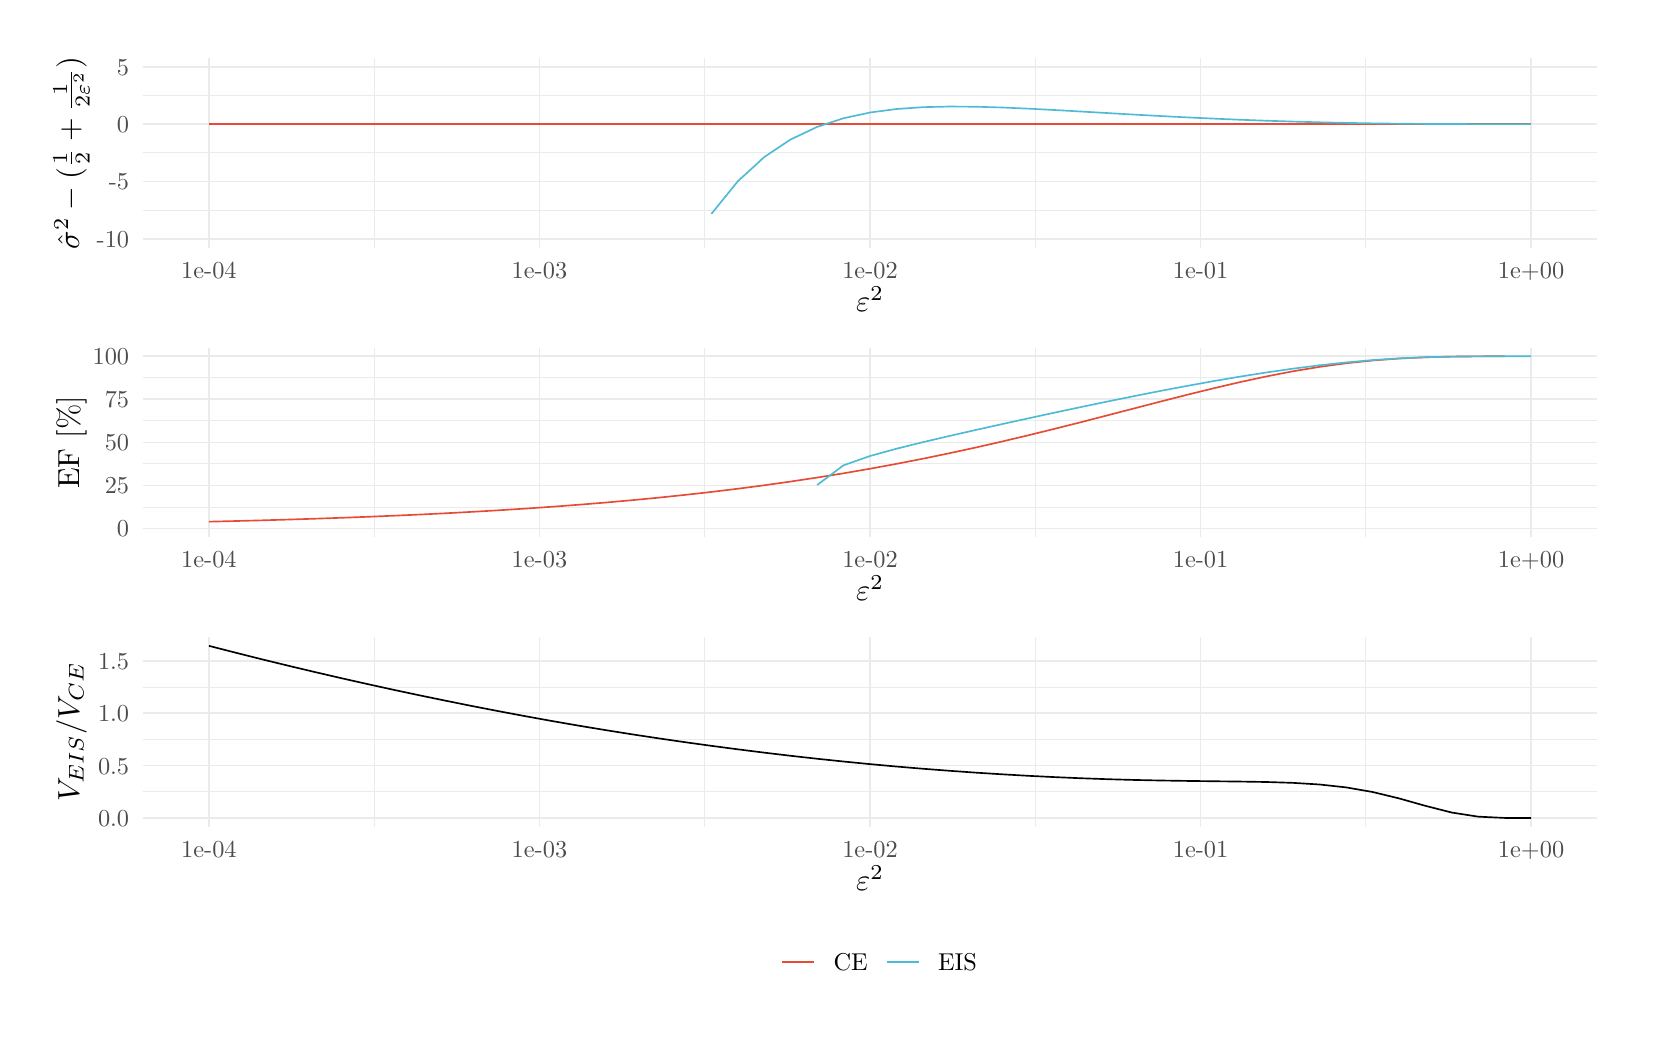
\begin{tikzpicture}[x=1pt,y=1pt]
\definecolor{fillColor}{RGB}{255,255,255}
\path[use as bounding box,fill=fillColor,fill opacity=0.00] (0,0) rectangle (578.16,361.35);
\begin{scope}
\path[clip] ( 41.61,281.90) rectangle (567.16,350.35);
\definecolor{drawColor}{gray}{0.92}

\path[draw=drawColor,line width= 0.3pt,line join=round] ( 41.61,295.39) --
	(567.16,295.39);

\path[draw=drawColor,line width= 0.3pt,line join=round] ( 41.61,316.13) --
	(567.16,316.13);

\path[draw=drawColor,line width= 0.3pt,line join=round] ( 41.61,336.87) --
	(567.16,336.87);

\path[draw=drawColor,line width= 0.3pt,line join=round] (125.22,281.90) --
	(125.22,350.35);

\path[draw=drawColor,line width= 0.3pt,line join=round] (244.66,281.90) --
	(244.66,350.35);

\path[draw=drawColor,line width= 0.3pt,line join=round] (364.11,281.90) --
	(364.11,350.35);

\path[draw=drawColor,line width= 0.3pt,line join=round] (483.55,281.90) --
	(483.55,350.35);

\path[draw=drawColor,line width= 0.6pt,line join=round] ( 41.61,285.02) --
	(567.16,285.02);

\path[draw=drawColor,line width= 0.6pt,line join=round] ( 41.61,305.76) --
	(567.16,305.76);

\path[draw=drawColor,line width= 0.6pt,line join=round] ( 41.61,326.50) --
	(567.16,326.50);

\path[draw=drawColor,line width= 0.6pt,line join=round] ( 41.61,347.24) --
	(567.16,347.24);

\path[draw=drawColor,line width= 0.6pt,line join=round] ( 65.50,281.90) --
	( 65.50,350.35);

\path[draw=drawColor,line width= 0.6pt,line join=round] (184.94,281.90) --
	(184.94,350.35);

\path[draw=drawColor,line width= 0.6pt,line join=round] (304.39,281.90) --
	(304.39,350.35);

\path[draw=drawColor,line width= 0.6pt,line join=round] (423.83,281.90) --
	(423.83,350.35);

\path[draw=drawColor,line width= 0.6pt,line join=round] (543.27,281.90) --
	(543.27,350.35);
\definecolor{drawColor}{RGB}{230,75,53}

\path[draw=drawColor,line width= 0.6pt,line join=round] ( 65.50,326.50) --
	( 75.06,326.50) --
	( 84.61,326.50) --
	( 94.17,326.50) --
	(103.72,326.50) --
	(113.28,326.50) --
	(122.83,326.50) --
	(132.39,326.50) --
	(141.94,326.50) --
	(151.50,326.50) --
	(161.05,326.50) --
	(170.61,326.50) --
	(180.16,326.50) --
	(189.72,326.50) --
	(199.28,326.50) --
	(208.83,326.50) --
	(218.39,326.50) --
	(227.94,326.50) --
	(237.50,326.50) --
	(247.05,326.50) --
	(256.61,326.50) --
	(266.16,326.50) --
	(275.72,326.50) --
	(285.27,326.50) --
	(294.83,326.50) --
	(304.39,326.50) --
	(313.94,326.50) --
	(323.50,326.50) --
	(333.05,326.50) --
	(342.61,326.50) --
	(352.16,326.50) --
	(361.72,326.50) --
	(371.27,326.50) --
	(380.83,326.50) --
	(390.38,326.50) --
	(399.94,326.50) --
	(409.50,326.50) --
	(419.05,326.50) --
	(428.61,326.50) --
	(438.16,326.50) --
	(447.72,326.50) --
	(457.27,326.50) --
	(466.83,326.50) --
	(476.38,326.50) --
	(485.94,326.50) --
	(495.49,326.50) --
	(505.05,326.50) --
	(514.61,326.50) --
	(524.16,326.50) --
	(533.72,326.50) --
	(543.27,326.50);
\definecolor{drawColor}{RGB}{77,187,213}

\path[draw=drawColor,line width= 0.6pt,line join=round] (247.05,294.04) --
	(256.61,305.84) --
	(266.16,314.59) --
	(275.72,320.96) --
	(285.27,325.49) --
	(294.83,328.62) --
	(304.39,330.69) --
	(313.94,331.95) --
	(323.50,332.62) --
	(333.05,332.85) --
	(342.61,332.78) --
	(352.16,332.50) --
	(361.72,332.08) --
	(371.27,331.58) --
	(380.83,331.03) --
	(390.38,330.48) --
	(399.94,329.93) --
	(409.50,329.41) --
	(419.05,328.92) --
	(428.61,328.48) --
	(438.16,328.07) --
	(447.72,327.72) --
	(457.27,327.41) --
	(466.83,327.15) --
	(476.38,326.94) --
	(485.94,326.77) --
	(495.49,326.65) --
	(505.05,326.56) --
	(514.61,326.52) --
	(524.16,326.50) --
	(533.72,326.50) --
	(543.27,326.50);
\end{scope}
\begin{scope}
\path[clip] (  0.00,  0.00) rectangle (578.16,361.35);
\definecolor{drawColor}{gray}{0.30}

\node[text=drawColor,anchor=base east,inner sep=0pt, outer sep=0pt, scale=  0.88] at ( 36.66,281.98) {-10};

\node[text=drawColor,anchor=base east,inner sep=0pt, outer sep=0pt, scale=  0.88] at ( 36.66,302.73) {-5};

\node[text=drawColor,anchor=base east,inner sep=0pt, outer sep=0pt, scale=  0.88] at ( 36.66,323.47) {0};

\node[text=drawColor,anchor=base east,inner sep=0pt, outer sep=0pt, scale=  0.88] at ( 36.66,344.21) {5};
\end{scope}
\begin{scope}
\path[clip] (  0.00,  0.00) rectangle (578.16,361.35);
\definecolor{drawColor}{gray}{0.30}

\node[text=drawColor,anchor=base,inner sep=0pt, outer sep=0pt, scale=  0.88] at ( 65.50,270.89) {1e-04};

\node[text=drawColor,anchor=base,inner sep=0pt, outer sep=0pt, scale=  0.88] at (184.94,270.89) {1e-03};

\node[text=drawColor,anchor=base,inner sep=0pt, outer sep=0pt, scale=  0.88] at (304.39,270.89) {1e-02};

\node[text=drawColor,anchor=base,inner sep=0pt, outer sep=0pt, scale=  0.88] at (423.83,270.89) {1e-01};

\node[text=drawColor,anchor=base,inner sep=0pt, outer sep=0pt, scale=  0.88] at (543.27,270.89) {1e+00};
\end{scope}
\begin{scope}
\path[clip] (  0.00,  0.00) rectangle (578.16,361.35);
\definecolor{drawColor}{RGB}{0,0,0}

\node[text=drawColor,anchor=base,inner sep=0pt, outer sep=0pt, scale=  1.10] at (304.39,258.86) {$\varepsilon^2$};
\end{scope}
\begin{scope}
\path[clip] (  0.00,  0.00) rectangle (578.16,361.35);
\definecolor{drawColor}{RGB}{0,0,0}

\node[text=drawColor,rotate= 90.00,anchor=base,inner sep=0pt, outer sep=0pt, scale=  1.10] at ( 18.58,316.13) {$\hat \sigma^2 - (\frac 1 2 + \frac 1 {2\varepsilon^2})$};
\end{scope}
\begin{scope}
\path[clip] ( 41.61,177.27) rectangle (567.16,245.72);
\definecolor{drawColor}{gray}{0.92}

\path[draw=drawColor,line width= 0.3pt,line join=round] ( 41.61,188.16) --
	(567.16,188.16);

\path[draw=drawColor,line width= 0.3pt,line join=round] ( 41.61,203.72) --
	(567.16,203.72);

\path[draw=drawColor,line width= 0.3pt,line join=round] ( 41.61,219.27) --
	(567.16,219.27);

\path[draw=drawColor,line width= 0.3pt,line join=round] ( 41.61,234.83) --
	(567.16,234.83);

\path[draw=drawColor,line width= 0.3pt,line join=round] (125.22,177.27) --
	(125.22,245.72);

\path[draw=drawColor,line width= 0.3pt,line join=round] (244.66,177.27) --
	(244.66,245.72);

\path[draw=drawColor,line width= 0.3pt,line join=round] (364.11,177.27) --
	(364.11,245.72);

\path[draw=drawColor,line width= 0.3pt,line join=round] (483.55,177.27) --
	(483.55,245.72);

\path[draw=drawColor,line width= 0.6pt,line join=round] ( 41.61,180.38) --
	(567.16,180.38);

\path[draw=drawColor,line width= 0.6pt,line join=round] ( 41.61,195.94) --
	(567.16,195.94);

\path[draw=drawColor,line width= 0.6pt,line join=round] ( 41.61,211.49) --
	(567.16,211.49);

\path[draw=drawColor,line width= 0.6pt,line join=round] ( 41.61,227.05) --
	(567.16,227.05);

\path[draw=drawColor,line width= 0.6pt,line join=round] ( 41.61,242.61) --
	(567.16,242.61);

\path[draw=drawColor,line width= 0.6pt,line join=round] ( 65.50,177.27) --
	( 65.50,245.72);

\path[draw=drawColor,line width= 0.6pt,line join=round] (184.94,177.27) --
	(184.94,245.72);

\path[draw=drawColor,line width= 0.6pt,line join=round] (304.39,177.27) --
	(304.39,245.72);

\path[draw=drawColor,line width= 0.6pt,line join=round] (423.83,177.27) --
	(423.83,245.72);

\path[draw=drawColor,line width= 0.6pt,line join=round] (543.27,177.27) --
	(543.27,245.72);
\definecolor{drawColor}{RGB}{230,75,53}

\path[draw=drawColor,line width= 0.6pt,line join=round] ( 65.50,182.84) --
	( 75.06,183.07) --
	( 84.61,183.32) --
	( 94.17,183.60) --
	(103.72,183.91) --
	(113.28,184.24) --
	(122.83,184.60) --
	(132.39,185.00) --
	(141.94,185.43) --
	(151.50,185.90) --
	(161.05,186.42) --
	(170.61,186.98) --
	(180.16,187.59) --
	(189.72,188.25) --
	(199.28,188.97) --
	(208.83,189.75) --
	(218.39,190.60) --
	(227.94,191.52) --
	(237.50,192.51) --
	(247.05,193.58) --
	(256.61,194.74) --
	(266.16,195.99) --
	(275.72,197.34) --
	(285.27,198.78) --
	(294.83,200.32) --
	(304.39,201.97) --
	(313.94,203.73) --
	(323.50,205.59) --
	(333.05,207.57) --
	(342.61,209.64) --
	(352.16,211.82) --
	(361.72,214.09) --
	(371.27,216.44) --
	(380.83,218.85) --
	(390.38,221.32) --
	(399.94,223.80) --
	(409.50,226.28) --
	(419.05,228.71) --
	(428.61,231.06) --
	(438.16,233.29) --
	(447.72,235.35) --
	(457.27,237.19) --
	(466.83,238.78) --
	(476.38,240.08) --
	(485.94,241.08) --
	(495.49,241.80) --
	(505.05,242.24) --
	(514.61,242.48) --
	(524.16,242.58) --
	(533.72,242.61);
\definecolor{drawColor}{RGB}{77,187,213}

\path[draw=drawColor,line width= 0.6pt,line join=round] (285.27,196.08) --
	(294.83,203.22) --
	(304.39,206.57) --
	(313.94,209.20) --
	(323.50,211.57) --
	(333.05,213.81) --
	(342.61,215.98) --
	(352.16,218.11) --
	(361.72,220.21) --
	(371.27,222.28) --
	(380.83,224.31) --
	(390.38,226.30) --
	(399.94,228.24) --
	(409.50,230.12) --
	(419.05,231.92) --
	(428.61,233.65) --
	(438.16,235.27) --
	(447.72,236.77) --
	(457.27,238.14) --
	(466.83,239.35) --
	(476.38,240.38) --
	(485.94,241.22) --
	(495.49,241.84) --
	(505.05,242.25) --
	(514.61,242.48) --
	(524.16,242.58) --
	(533.72,242.61) --
	(543.27,242.61);
\end{scope}
\begin{scope}
\path[clip] (  0.00,  0.00) rectangle (578.16,361.35);
\definecolor{drawColor}{gray}{0.30}

\node[text=drawColor,anchor=base east,inner sep=0pt, outer sep=0pt, scale=  0.88] at ( 36.66,177.35) {0};

\node[text=drawColor,anchor=base east,inner sep=0pt, outer sep=0pt, scale=  0.88] at ( 36.66,192.91) {25};

\node[text=drawColor,anchor=base east,inner sep=0pt, outer sep=0pt, scale=  0.88] at ( 36.66,208.46) {50};

\node[text=drawColor,anchor=base east,inner sep=0pt, outer sep=0pt, scale=  0.88] at ( 36.66,224.02) {75};

\node[text=drawColor,anchor=base east,inner sep=0pt, outer sep=0pt, scale=  0.88] at ( 36.66,239.58) {100};
\end{scope}
\begin{scope}
\path[clip] (  0.00,  0.00) rectangle (578.16,361.35);
\definecolor{drawColor}{gray}{0.30}

\node[text=drawColor,anchor=base,inner sep=0pt, outer sep=0pt, scale=  0.88] at ( 65.50,166.26) {1e-04};

\node[text=drawColor,anchor=base,inner sep=0pt, outer sep=0pt, scale=  0.88] at (184.94,166.26) {1e-03};

\node[text=drawColor,anchor=base,inner sep=0pt, outer sep=0pt, scale=  0.88] at (304.39,166.26) {1e-02};

\node[text=drawColor,anchor=base,inner sep=0pt, outer sep=0pt, scale=  0.88] at (423.83,166.26) {1e-01};

\node[text=drawColor,anchor=base,inner sep=0pt, outer sep=0pt, scale=  0.88] at (543.27,166.26) {1e+00};
\end{scope}
\begin{scope}
\path[clip] (  0.00,  0.00) rectangle (578.16,361.35);
\definecolor{drawColor}{RGB}{0,0,0}

\node[text=drawColor,anchor=base,inner sep=0pt, outer sep=0pt, scale=  1.10] at (304.39,154.22) {$\varepsilon^2$};
\end{scope}
\begin{scope}
\path[clip] (  0.00,  0.00) rectangle (578.16,361.35);
\definecolor{drawColor}{RGB}{0,0,0}

\node[text=drawColor,rotate= 90.00,anchor=base,inner sep=0pt, outer sep=0pt, scale=  1.10] at ( 18.58,211.49) {EF [\%]};
\end{scope}
\begin{scope}
\path[clip] ( 41.61, 72.64) rectangle (567.16,141.09);
\definecolor{drawColor}{gray}{0.92}

\path[draw=drawColor,line width= 0.3pt,line join=round] ( 41.61, 85.22) --
	(567.16, 85.22);

\path[draw=drawColor,line width= 0.3pt,line join=round] ( 41.61,104.15) --
	(567.16,104.15);

\path[draw=drawColor,line width= 0.3pt,line join=round] ( 41.61,123.08) --
	(567.16,123.08);

\path[draw=drawColor,line width= 0.3pt,line join=round] (125.22, 72.64) --
	(125.22,141.09);

\path[draw=drawColor,line width= 0.3pt,line join=round] (244.66, 72.64) --
	(244.66,141.09);

\path[draw=drawColor,line width= 0.3pt,line join=round] (364.11, 72.64) --
	(364.11,141.09);

\path[draw=drawColor,line width= 0.3pt,line join=round] (483.55, 72.64) --
	(483.55,141.09);

\path[draw=drawColor,line width= 0.6pt,line join=round] ( 41.61, 75.75) --
	(567.16, 75.75);

\path[draw=drawColor,line width= 0.6pt,line join=round] ( 41.61, 94.68) --
	(567.16, 94.68);

\path[draw=drawColor,line width= 0.6pt,line join=round] ( 41.61,113.61) --
	(567.16,113.61);

\path[draw=drawColor,line width= 0.6pt,line join=round] ( 41.61,132.54) --
	(567.16,132.54);

\path[draw=drawColor,line width= 0.6pt,line join=round] ( 65.50, 72.64) --
	( 65.50,141.09);

\path[draw=drawColor,line width= 0.6pt,line join=round] (184.94, 72.64) --
	(184.94,141.09);

\path[draw=drawColor,line width= 0.6pt,line join=round] (304.39, 72.64) --
	(304.39,141.09);

\path[draw=drawColor,line width= 0.6pt,line join=round] (423.83, 72.64) --
	(423.83,141.09);

\path[draw=drawColor,line width= 0.6pt,line join=round] (543.27, 72.64) --
	(543.27,141.09);
\definecolor{drawColor}{RGB}{0,0,0}

\path[draw=drawColor,line width= 0.6pt,line join=round] ( 65.50,137.97) --
	( 75.06,135.52) --
	( 84.61,133.12) --
	( 94.17,130.79) --
	(103.72,128.52) --
	(113.28,126.30) --
	(122.83,124.15) --
	(132.39,122.05) --
	(141.94,120.02) --
	(151.50,118.05) --
	(161.05,116.13) --
	(170.61,114.28) --
	(180.16,112.49) --
	(189.72,110.76) --
	(199.28,109.10) --
	(208.83,107.52) --
	(218.39,106.00) --
	(227.94,104.55) --
	(237.50,103.16) --
	(247.05,101.84) --
	(256.61,100.58) --
	(266.16, 99.38) --
	(275.72, 98.24) --
	(285.27, 97.17) --
	(294.83, 96.17) --
	(304.39, 95.23) --
	(313.94, 94.36) --
	(323.50, 93.56) --
	(333.05, 92.83) --
	(342.61, 92.15) --
	(352.16, 91.55) --
	(361.72, 91.00) --
	(371.27, 90.53) --
	(380.83, 90.12) --
	(390.38, 89.78) --
	(399.94, 89.51) --
	(409.50, 89.31) --
	(419.05, 89.16) --
	(428.61, 89.04) --
	(438.16, 88.93) --
	(447.72, 88.77) --
	(457.27, 88.46) --
	(466.83, 87.87) --
	(476.38, 86.83) --
	(485.94, 85.17) --
	(495.49, 82.86) --
	(505.05, 80.16) --
	(514.61, 77.73) --
	(524.16, 76.25) --
	(533.72, 75.79) --
	(543.27, 75.75);
\end{scope}
\begin{scope}
\path[clip] (  0.00,  0.00) rectangle (578.16,361.35);
\definecolor{drawColor}{gray}{0.30}

\node[text=drawColor,anchor=base east,inner sep=0pt, outer sep=0pt, scale=  0.88] at ( 36.66, 72.72) {0.0};

\node[text=drawColor,anchor=base east,inner sep=0pt, outer sep=0pt, scale=  0.88] at ( 36.66, 91.65) {0.5};

\node[text=drawColor,anchor=base east,inner sep=0pt, outer sep=0pt, scale=  0.88] at ( 36.66,110.58) {1.0};

\node[text=drawColor,anchor=base east,inner sep=0pt, outer sep=0pt, scale=  0.88] at ( 36.66,129.51) {1.5};
\end{scope}
\begin{scope}
\path[clip] (  0.00,  0.00) rectangle (578.16,361.35);
\definecolor{drawColor}{gray}{0.30}

\node[text=drawColor,anchor=base,inner sep=0pt, outer sep=0pt, scale=  0.88] at ( 65.50, 61.63) {1e-04};

\node[text=drawColor,anchor=base,inner sep=0pt, outer sep=0pt, scale=  0.88] at (184.94, 61.63) {1e-03};

\node[text=drawColor,anchor=base,inner sep=0pt, outer sep=0pt, scale=  0.88] at (304.39, 61.63) {1e-02};

\node[text=drawColor,anchor=base,inner sep=0pt, outer sep=0pt, scale=  0.88] at (423.83, 61.63) {1e-01};

\node[text=drawColor,anchor=base,inner sep=0pt, outer sep=0pt, scale=  0.88] at (543.27, 61.63) {1e+00};
\end{scope}
\begin{scope}
\path[clip] (  0.00,  0.00) rectangle (578.16,361.35);
\definecolor{drawColor}{RGB}{0,0,0}

\node[text=drawColor,anchor=base,inner sep=0pt, outer sep=0pt, scale=  1.10] at (304.39, 49.59) {$\varepsilon^2$};
\end{scope}
\begin{scope}
\path[clip] (  0.00,  0.00) rectangle (578.16,361.35);
\definecolor{drawColor}{RGB}{0,0,0}

\node[text=drawColor,rotate= 90.00,anchor=base,inner sep=0pt, outer sep=0pt, scale=  1.10] at ( 18.58,106.86) {$V_{EIS} / V_{CE}$};
\end{scope}
\begin{scope}
\path[clip] (  0.00,  0.00) rectangle (578.16,361.35);
\definecolor{drawColor}{RGB}{230,75,53}

\path[draw=drawColor,line width= 0.6pt,line join=round] (272.68, 23.73) -- (284.24, 23.73);
\end{scope}
\begin{scope}
\path[clip] (  0.00,  0.00) rectangle (578.16,361.35);
\definecolor{drawColor}{RGB}{77,187,213}

\path[draw=drawColor,line width= 0.6pt,line join=round] (310.48, 23.73) -- (322.04, 23.73);
\end{scope}
\begin{scope}
\path[clip] (  0.00,  0.00) rectangle (578.16,361.35);
\definecolor{drawColor}{RGB}{0,0,0}

\node[text=drawColor,anchor=base west,inner sep=0pt, outer sep=0pt, scale=  0.88] at (291.19, 20.70) {CE};
\end{scope}
\begin{scope}
\path[clip] (  0.00,  0.00) rectangle (578.16,361.35);
\definecolor{drawColor}{RGB}{0,0,0}

\node[text=drawColor,anchor=base west,inner sep=0pt, outer sep=0pt, scale=  0.88] at (328.98, 20.70) {EIS};
\end{scope}
\end{tikzpicture}
